\documentclass[conference]{IEEEtran}
\IEEEoverridecommandlockouts
\usepackage{cite}
\usepackage{amsmath,amssymb,amsfonts}
\usepackage{algorithmic}
\usepackage{graphicx}
\usepackage{textcomp}
\usepackage{xcolor}
\usepackage{url}
\usepackage{booktabs}
\def\BibTeX{{\rm B\kern-.05em{\sc i\kern-.025em b}\kern-.08em
    T\kern-.1667em\lower.7ex\hbox{E}\kern-.125emX}}

\begin{document}

\title{A Decoupled Vector Coprocessor for RISC-V \\
{\footnotesize ECE/COS 475 Final Project, Spring 2026}}

\author{\IEEEauthorblockN{Max Machado}
\IEEEauthorblockA{\textit{Department of Electrical and Computer Engineering} \\
\textit{Princeton University}\\
Princeton, NJ \\
}
\and
\IEEEauthorblockN{Connor Brown}
\IEEEauthorblockA{\textit{Department of Electrical and Computer Engineering} \\
\textit{Princeton University}\\
Princeton, NJ \\
}
}

\maketitle

\begin{abstract}
We design and evaluate a decoupled vector coprocessor for the
five-stage RISC-V processor developed in ECE/COS 475 labs. The unit
implements a 32-instruction custom vector ISA with eight
$32 \times 32$-bit vector registers, a four-entry command queue,
predicated execution via a mask register, strip-mining via SETVL,
and reductions back to the scalar register file. We build two
variants: a baseline single-ALU design (\textit{riscvvec}) and a
Cray-style chained variant (\textit{riscvvec-chained}) with a 3R/2W
vector register file, two ALUs, dual-issue control, and a forwarding
mux that allows a producer/consumer pair to run in roughly one chime.
Across six kernels we measure 1.9$\times$ to 9.0$\times$ speedup over
the scalar 5-stage baseline, with chaining adding up to a further
13\% on dependent kernels such as DAXPY. The largest gains occur on
LINPACK (9.0$\times$), where loop overhead dominates the scalar
runtime. A chain-depth microbenchmark confirms the chaining
mechanism halves the cost of every consecutive RAW-dependent op pair.
\end{abstract}

\section{Introduction}
Many scientific and signal-processing kernels operate on long arrays
in regular patterns. A scalar processor running such code spends most
of its energy and clock cycles on overhead rather than useful math:
fetching instructions, decoding them, incrementing loop counters,
checking branch conditions, and reading and writing the register
file once per element. A vector instruction set sidesteps almost all
of that. A single instruction commands an operation over an entire
array, the hardware walks the elements internally, and the scalar
front-end is free to do other work while it runs.

This term project explores that idea by building a decoupled vector
coprocessor that attaches to the five-stage in-order RISC-V core we
built across ECE/COS 475 Labs 1--4. We then build a second variant
that adds operation chaining, which the textbook
\cite{hp_book} highlights as the technique that makes early
vector machines such as the Cray-1 \cite{cray1} so effective on
chained producer/consumer code patterns. The contributions of this
report are:
\begin{itemize}
\item A 32-instruction custom vector ISA layered on the RISC-V
  custom-0 opcode, covering vector-vector and vector-scalar
  arithmetic, unit and strided memory access, predicated execution,
  configuration, and reductions.
\item Two synthesizable RTL designs in Verilog: a baseline single-ALU
  decoupled vector unit, and a chained variant with a 3R/2W register
  file, two ALUs, and producer-to-consumer forwarding.
\item A full evaluation against three non-vector reference designs
  (5-stage bypass, longer pipeline, OOO dual-issue) on six kernels,
  plus parametric sweeps over problem size, command queue depth, and
  chain depth.
\end{itemize}

\section{Background and Related Work}
Modern data-parallel acceleration follows three broad lineages
\cite{hp_book}: classical vector architectures, multimedia SIMD
extensions, and GPU-style multithreaded SIMD. Our work follows the
first.

\textbf{Classical vector architectures.} The Cray-1 \cite{cray1}
established the basic vector machine recipe used in the textbook's
VMIPS exposition: a vector register file, a small number of pipelined
functional units, vector load/store with strides, and chaining
between dependent vector operations. The textbook's analysis
\cite[Ch.~4]{hp_book} of DAXPY motivates our project: a vector
encoding reduces the dynamic instruction count of an inner loop by
roughly 100$\times$ relative to the equivalent scalar code, because
loop control collapses into a single vector-length register and the
remaining instructions amortize across all elements.

\textbf{SIMD extensions.} Intel's MMX, SSE, and AVX series
\cite{avx_isa} take a different approach: fixed-width operand
bundles in opcode form, no vector-length register, and limited
support for strided access or predication. SIMD extensions are
easier to add to a scalar core but harder for compilers to target.
Our design follows the cleaner vector-architecture model since it is
the one developed in lecture.

\textbf{GPU-style SIMD.} GPUs \cite{nvidia_fermi} take vector ideas
further by combining wide SIMD lanes with hardware multithreading and
divergence handling. Their resource demands (large register files,
many lanes, scratchpad memory) put them out for this project, but the basic abstraction --- a single instruction
operating over many data elements --- is the same.

\textbf{Decoupled access/execute.} Smith's decoupled access/execute
architecture \cite{smith_dae} introduced the idea of letting an
asynchronous unit consume an instruction stream queued by the main
core. We use the same val/rdy queue pattern at the boundary between
our scalar core and the vector unit.

\textbf{Modern open-source vector ISAs.} The RISC-V Vector extension
\cite{rvv} is now standardized with variable-length vector
registers and a more comprehensive instruction set than our implementation. Hardware
implementations such as Hwacha \cite{hwacha} and Ara \cite{ara}
target the same general decoupled-coprocessor pattern at greater
scale and complexity. We use a custom ISA rather than RVV because
the latter's encoding density and configuration model are larger
than what we could implement in our limited time frame (2 weeks).

\section{System Architecture}
The full system, shown in Fig.~\ref{fig:sysarch}, consists of an
unmodified five-stage scalar pipeline (the \textit{riscvbyp} design
from Lab 2 with full bypassing), an attached vector coprocessor
(the \textit{VecUnit}), and a shared data memory port arbitrated
between the two.

\begin{figure}[t]
\centerline{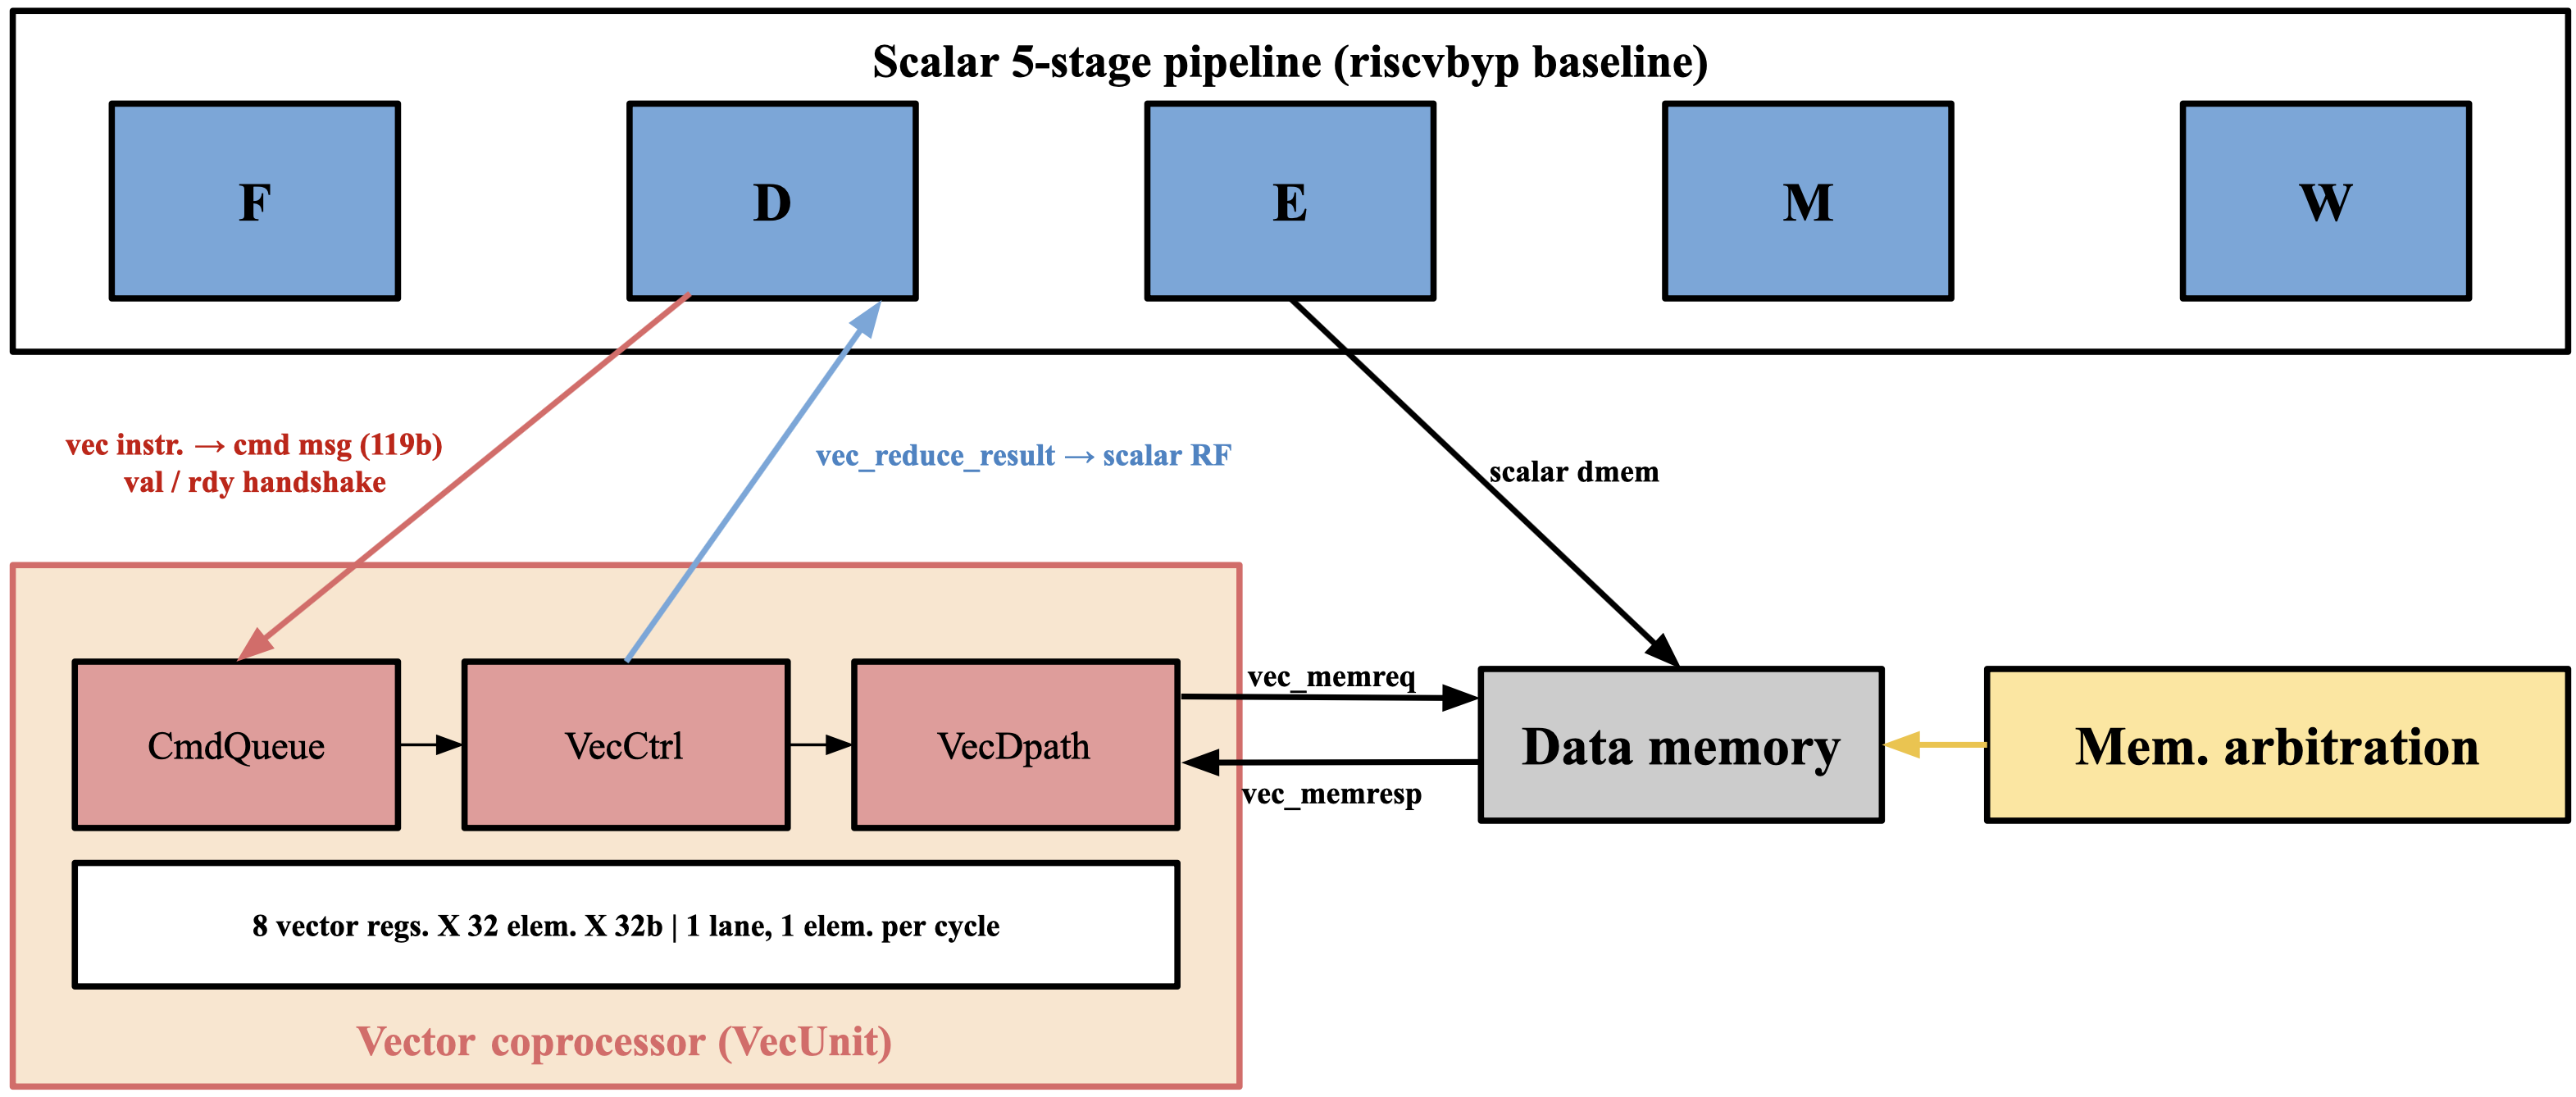
\includegraphics[width=\columnwidth]{media/system-arch.png}}
\caption{System architecture. The scalar pipeline dispatches a
packed 119-bit command message to the VecUnit at decode and
continues. The VecUnit walks elements internally and arbitrates with
the scalar core for memory.}
\label{fig:sysarch}
\end{figure}

\subsection{Scalar/Vector Decoupling}
When the scalar decode stage sees a vector opcode, it does not
execute it in the normal pipeline. Instead, it packs the relevant
fields --- category, opcode, vd/vs1/vs2 vector register addresses,
optional scalar operand from the integer register file, base address,
stride, and a destination scalar register for reductions --- into a
single 119-bit command message and pushes it into the vector
coprocessor's command queue over a val/rdy interface. The scalar
pipeline is then free to keep fetching, including dispatching more
vector instructions, until either the queue fills up or the program
issues a VFENCE.

This decoupling is the main feature of our project's design: the scalar
pipeline does not stall waiting for vector work to complete unless
the program explicitly synchronizes. As a result, vector loops that
take hundreds of cycles to run can overlap with whatever scalar work
follows them.

\subsection{VecUnit Internals}
Fig.~\ref{fig:vecunit} shows the inside of the vector unit. The
relevant components are:
\begin{itemize}
\item A four-entry FIFO command queue (\textit{VecCmdQueue}).
\item A finite-state-machine controller (\textit{VecCtrl}) that
  walks element indices and drives every control signal in the
  datapath. Its states are IDLE, EXEC (vector-vector and
  vector-scalar arithmetic), LOAD/LWAIT (vector loads), STORE
  (vector stores), and REDUCE (reductions back to a scalar
  register).
\item A vector register file (VRF) of $8 \times 32$ 32-bit
  elements, with two read ports and one write port in the
  baseline design.
\item A single-lane ALU (\textit{VecALU}) supporting integer add,
  sub, mul, div, rem, bitwise logic, shifts, and the six signed
  comparisons.
\item A 32-bit mask register that gates writes elementwise. It is
  set by VS-comparison instructions and cleared by CVM.
\item Stride logic for VLWS / VSWS that increments the memory
  address by an arbitrary scalar each cycle rather than a fixed 4.
\end{itemize}

\begin{figure}[t]
\centerline{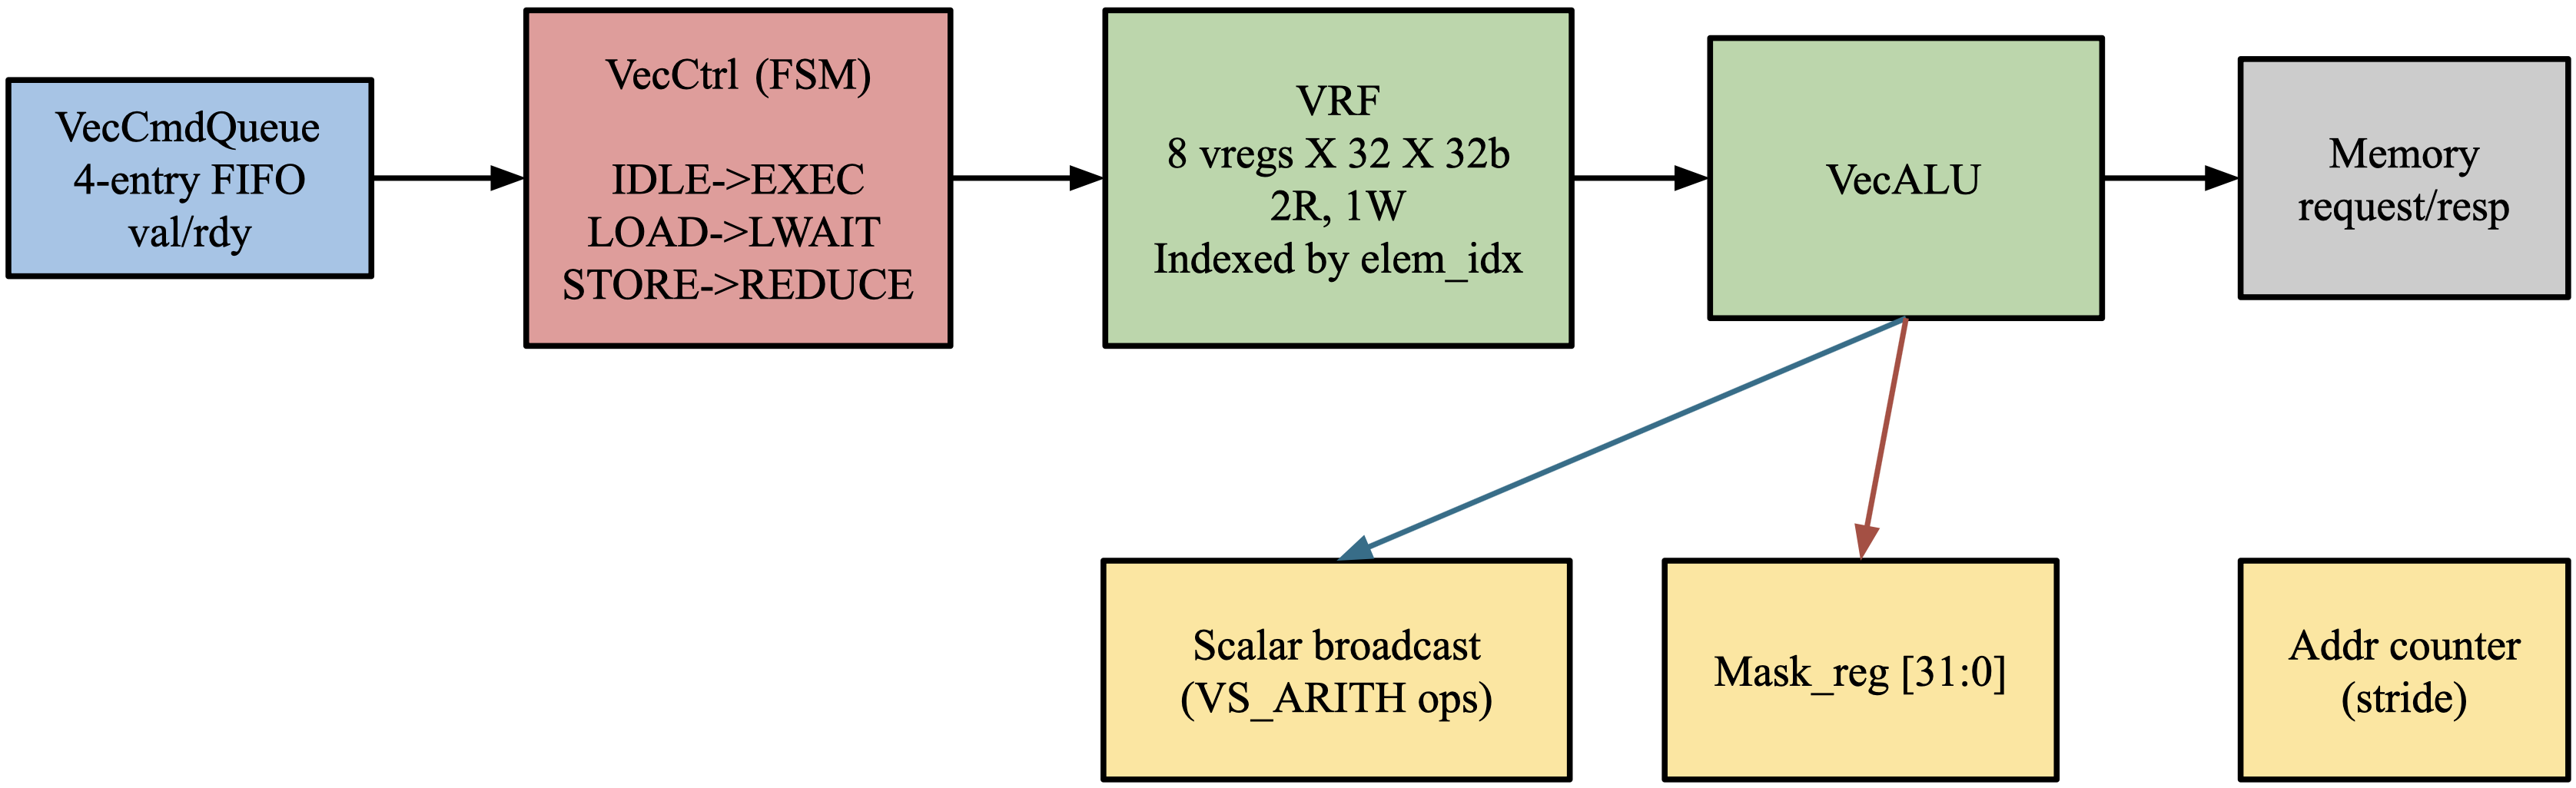
\includegraphics[width=\columnwidth]{media/vecunit-internals.png}}
\caption{Internal structure of the vector coprocessor. The FSM walks
elements one per cycle through a single ALU and writes results back
into the VRF. Mask register gates writes for predicated execution.}
\label{fig:vecunit}
\end{figure}

\subsection{Vector ISA}
We allocate the RISC-V \texttt{custom-0} opcode (\texttt{0x0B}) and
encode 32 instructions in R-type form with the category in
\texttt{funct3}:

\begin{itemize}
\item \textbf{VV arithmetic} (11 ops): VVADD/SUB/MUL/DIV/REM,
  VVAND/OR/XOR, VVSLL/SRL/SRA.
\item \textbf{VS arithmetic} (5 ops): VSADD/SUB/MUL/DIV/REM, with
  the scalar broadcast from the integer register file.
\item \textbf{Vector memory} (4 ops): VLW, VSW, VLWS, VSWS (unit and
  strided).
\item \textbf{Configuration} (3 ops): SETVL (clamps a requested
  length to VLMAX = 32 and writes the active length back to a scalar
  register), CVM (clear vector mask), and VFENCE (block scalar
  decode until the vector unit drains).
\item \textbf{Comparison} (6 ops): VSEQ/SLT/SLE/SGT/SGE/SNE, each
  setting one bit of the mask register per element.
\item \textbf{Reductions} (3 ops): VREDSUM, VREDAND, VREDOR, which
  fold a vector down to a scalar via an accumulator and write the
  result through a dedicated port to the scalar register file.
\end{itemize}

Strip-mining (handling vectors longer than VLMAX = 32) is done in
software by the assembly programmer or compiler: the kernel calls SETVL with the residual length each
iteration of an outer loop, then issues vector instructions at the
returned active length, then a VFENCE before advancing pointers.
This mirrors the strip-mining pattern in \cite[\S 4.2]{hp_book}.

\subsection{Chained Variant}
The chained version (Fig.~\ref{fig:chaining}) modifies three things
to enable a producer/consumer vector pair to overlap. First, the VRF
gets a third read port and a second write port. Second, the controller
is dual-issue: it can latch a producer command and a consumer command
on the same cycle from the queue and walk both element indices in
lockstep. Third, the consumer ALU's input mux can take its operand
from either the VRF read port or directly from the producer ALU's
combinational output, sidestepping the wait for a write-then-read of
the VRF slot.

The controller still detects and serializes hazards that chaining
cannot legally cover: WAW (both ops write the same vd), WAR (the
consumer reads what the producer would overwrite in non-RAW slots),
or shape mismatches such as a chained pair that includes a memory
operation, a reduction, or a comparison. In those cases the second
op falls back to ordinary serial issue.

\begin{figure}[t]
\centerline{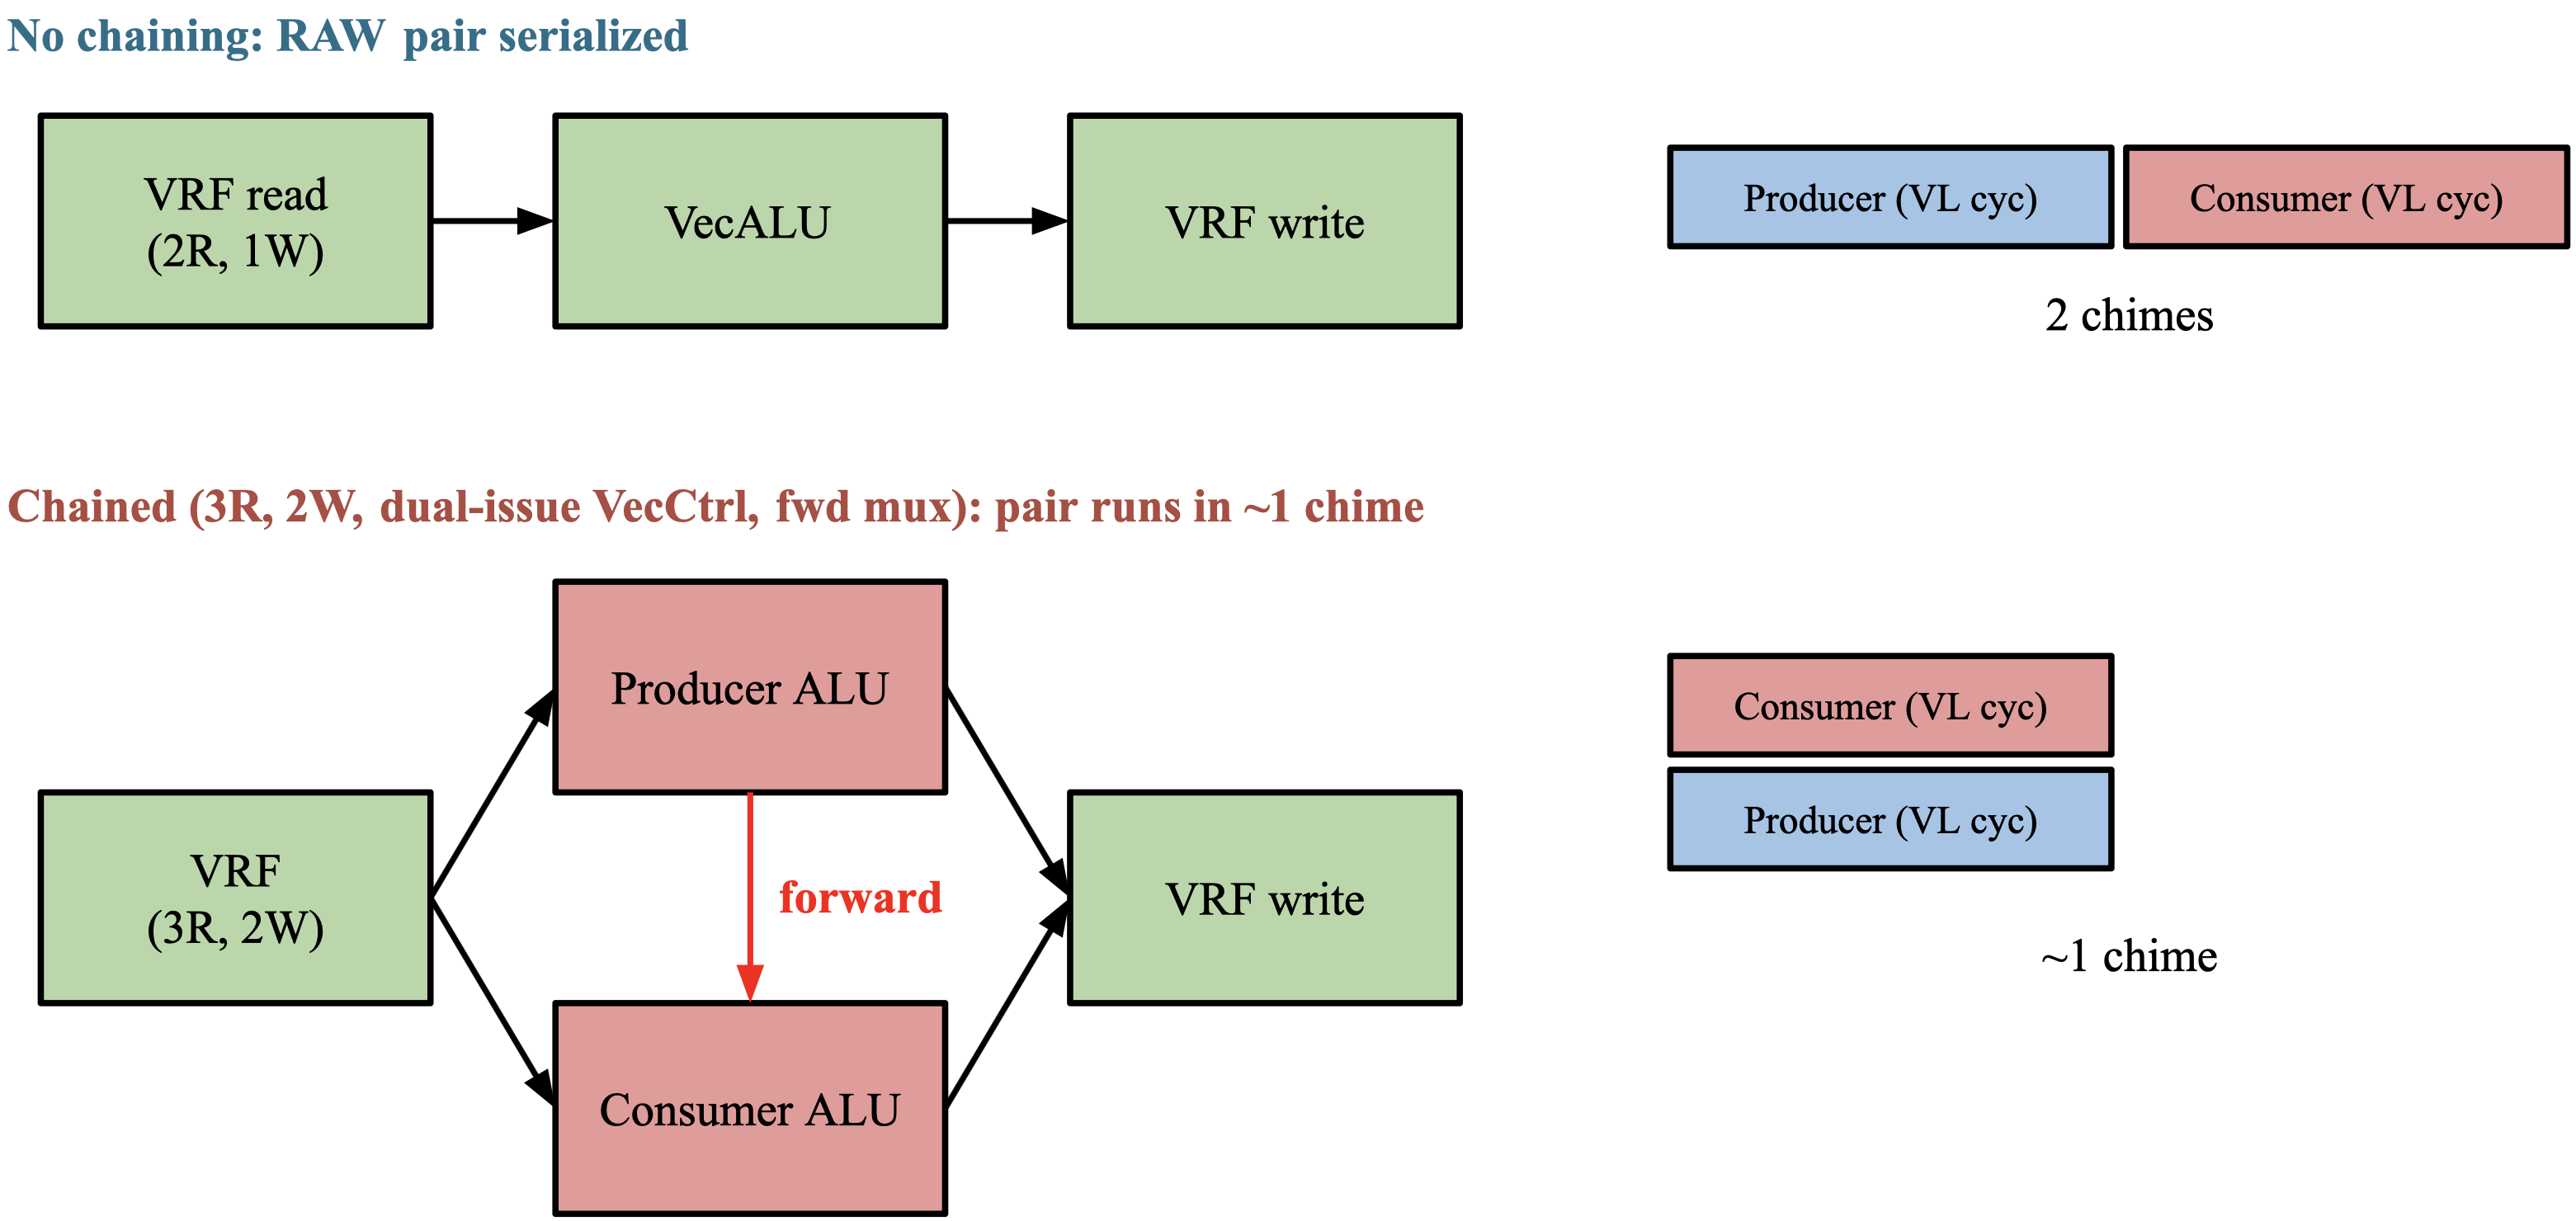
\includegraphics[width=\columnwidth]{media/chaining.png}}
\caption{Chaining mechanism. Top: the baseline serializes a
RAW-dependent pair across two chimes. Bottom: the chained design
forwards the producer's element output directly into the consumer
ALU and runs both in roughly one chime.}
\label{fig:chaining}
\end{figure}

\section{Methodology}
We evaluate against three non-vector reference designs, all reused
from earlier labs: \textit{riscvbyp} (5-stage with full bypassing,
the speedup denominator), \textit{riscvlong} (longer pipeline with
single-cycle multiplier), and \textit{riscvooo} (out-of-order dual-issue
from Lab 4).

We use six kernels reused from the lab benchmark harness, with the
inner loops rewritten in our vector ISA where applicable:
\begin{itemize}
\item \textbf{vvadd} --- elementwise array add. The simplest sanity
  check; isolates dispatch and load/store overhead.
\item \textbf{saxpy} --- scales an array by a constant and adds it
  to another. The textbook's canonical chaining target.
\item \textbf{daxpy} --- the same access pattern with longer arrays
  and an N-sweep so we can measure scaling behavior.
\item \textbf{linpack} --- Gaussian elimination on a $16 \times 16$
  matrix; mixes strided loads, scalar broadcasts, and accumulating
  updates.
\item \textbf{vvmul} --- elementwise array multiply, similar to
  vvadd but with the integer multiplier as the bottleneck on scalar
  designs.
\item \textbf{dotprod} --- sum-of-products via VVMUL into a temporary
  vector and then VREDSUM, exercising both arithmetic and reduction.
\end{itemize}
For lengths above VLMAX = 32 we strip-mine in software, calling
SETVL/VFENCE at the strip boundary so that every vectorized batch
exercises the scalar/coprocessor handshake. All variants pass the
existing checks from previous labs; this catches any
miscompiled inner loop or mishandled mask immediately.

We measure cycle count directly from the testbench. Functional
correctness is verified. For clarity, we note that the VecALU
operates on 32-bit integers only; the ``S'' and ``D'' in
saxpy/daxpy refer to the AXPY access pattern, not single or
double precision (no FP unit was implemented in this project due to time).

\section{Results and Analysis}
\subsection{Speedup over scalar baseline}
Fig.~\ref{fig:speedup} summarizes speedup over \textit{riscvbyp}
across all six kernels. The vector designs win across the board, by
margins that depend strongly on how compute-bound the kernel is.

\begin{figure}[t]
\centerline{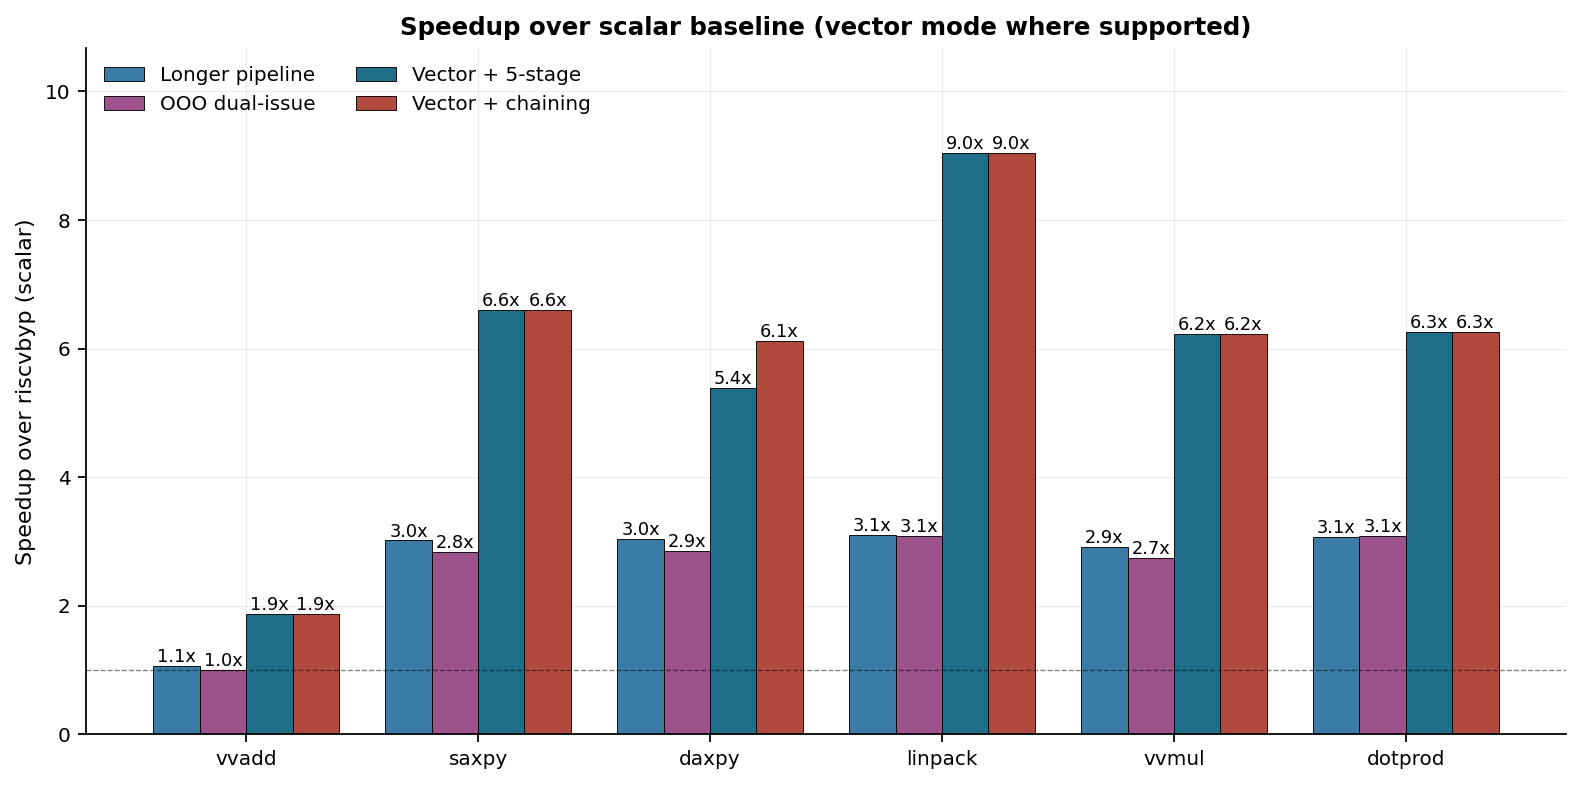
\includegraphics[width=\columnwidth]{media/speedup.png}}
\caption{Speedup of each design over the 5-stage scalar baseline.
Vector designs show speedups on every kernel; chaining helps most kernels on DAXPY.}
\label{fig:speedup}
\end{figure}

\textbf{vvadd} sees only 1.9$\times$. This is the kernel's natural
ceiling: there is essentially no compute (one add per element) so
the runtime is dominated by memory traffic, which is the same for
scalar and vector code. The performance bumpy is solely due to the removal of the scalar loop
overhead.

\textbf{saxpy, vvmul, dotprod} all sit around 6$\times$. Each element goes through one multiply plus an add or reduction step. The scalar core pays for at least one instruction per cycle. Our vector design amortizes this loop control overhead to nearly zero per element.

\textbf{daxpy} reaches 5.4$\times$ in the baseline and 6.1$\times$
with chaining --- a 13\% improvement which is directly attributable to the
producer/consumer overlap of MULVS and VVADD on every element.

\textbf{linpack} hits 9.0$\times$, the largest gain. LINPACK has
both arithmetic intensity (a multiply, an add, and a store per inner
iteration) and heavy loop overhead (nested counters, address
recomputation, branch comparison) that our vector ISA removes entirely.

The non-vector designs (longer pipeline, OOO) provide the expected
1--3$\times$ improvements but are nowhere near competitive on
data-parallel kernels.

\subsection{Throughput}
Fig.~\ref{fig:throughput} reframes the same data as ops per cycle
and makes the per-cycle work density of vector mode clearer.
Scalar designs sit between 0.02 and 0.07 ops/cycle; vector mode
reaches 0.13--0.38, with LINPACK pushing past 0.38 because it does
several useful operations per inner iteration.

\begin{figure}[t]
\centerline{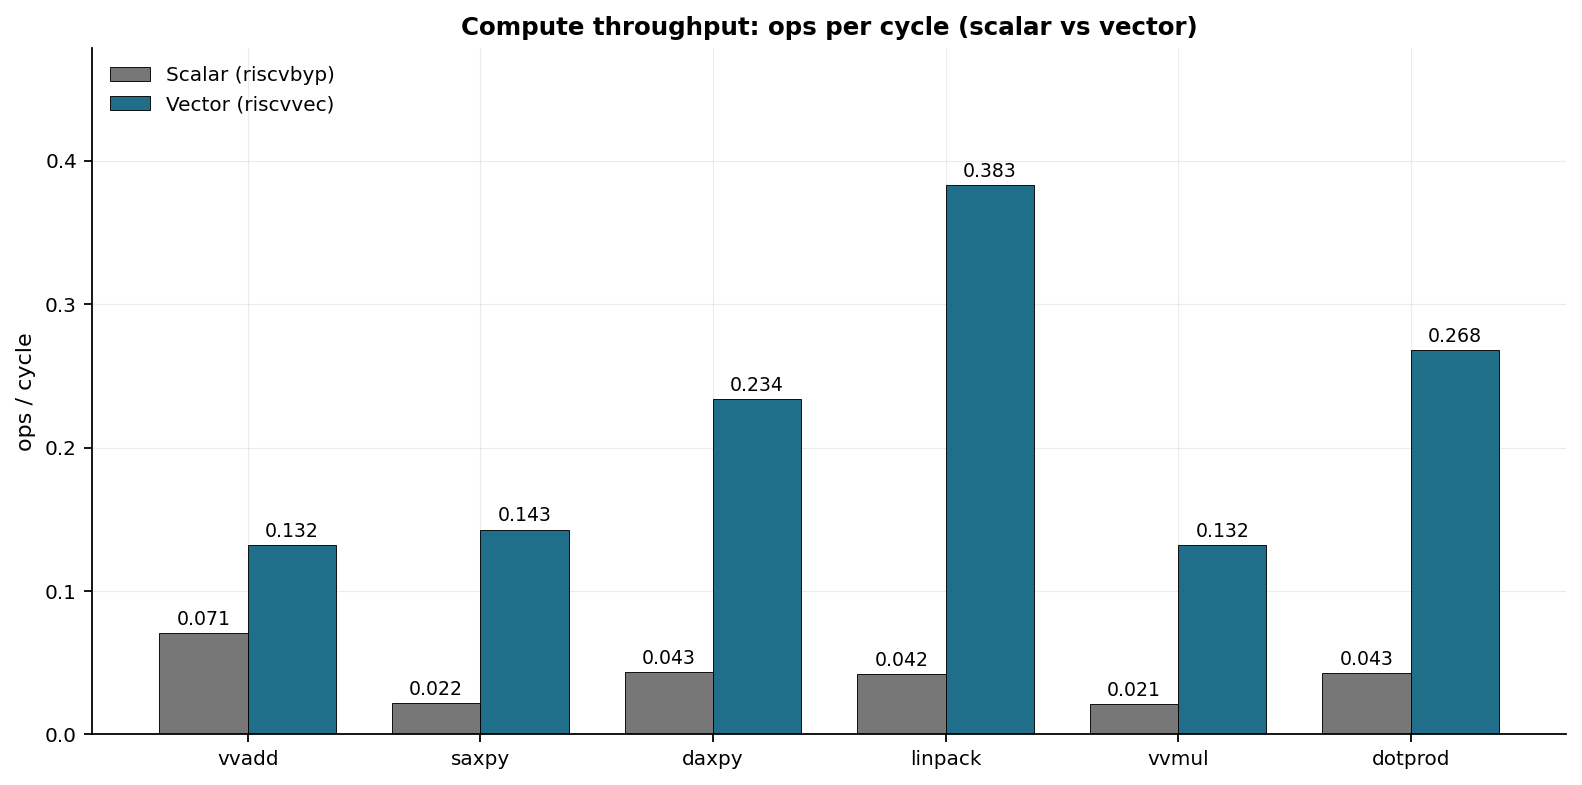
\includegraphics[width=\columnwidth]{media/throughput.png}}
\caption{Ops per cycle, scalar vs.~vector.}
\label{fig:throughput}
\end{figure}

\subsection{Scaling}
Fig.~\ref{fig:daxpy_scaling} sweeps DAXPY length over $N = 16, 32,
\ldots, 256$, showing all five designs scale linearly in $N$ (with
log-log slope $\approx 1$) but at very different intercepts and
slopes. The vector designs maintain a roughly constant cycle gap
below the scalar designs as $N$ grows, meaning the speedup ratio is
preserved across problem sizes. Fig.~\ref{fig:linpack_scaling}
repeats this for LINPACK across $N \in \{4, 8, 16, 32\}$ and shows
the same shape: vector and chained designs are stably below scalar
across all matrix dimensions, and OOO dual-issue overlaps the
longer-pipeline curve closely.

\begin{figure}[t]
\centerline{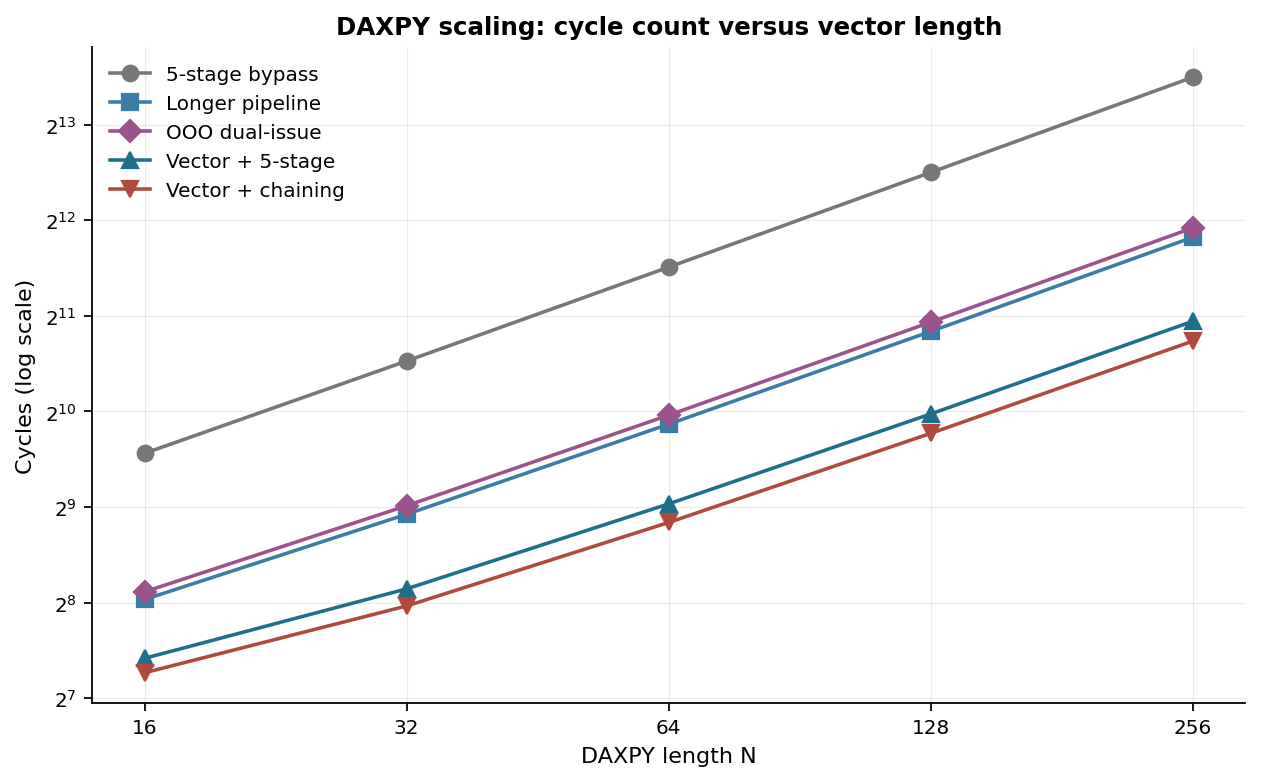
\includegraphics[width=\columnwidth]{media/daxpy-scaling.png}}
\caption{DAXPY scaling. The vector advantage is preserved across N
and chaining provides a consistent additional performance gain.}
\label{fig:daxpy_scaling}
\end{figure}

\begin{figure}[t]
\centerline{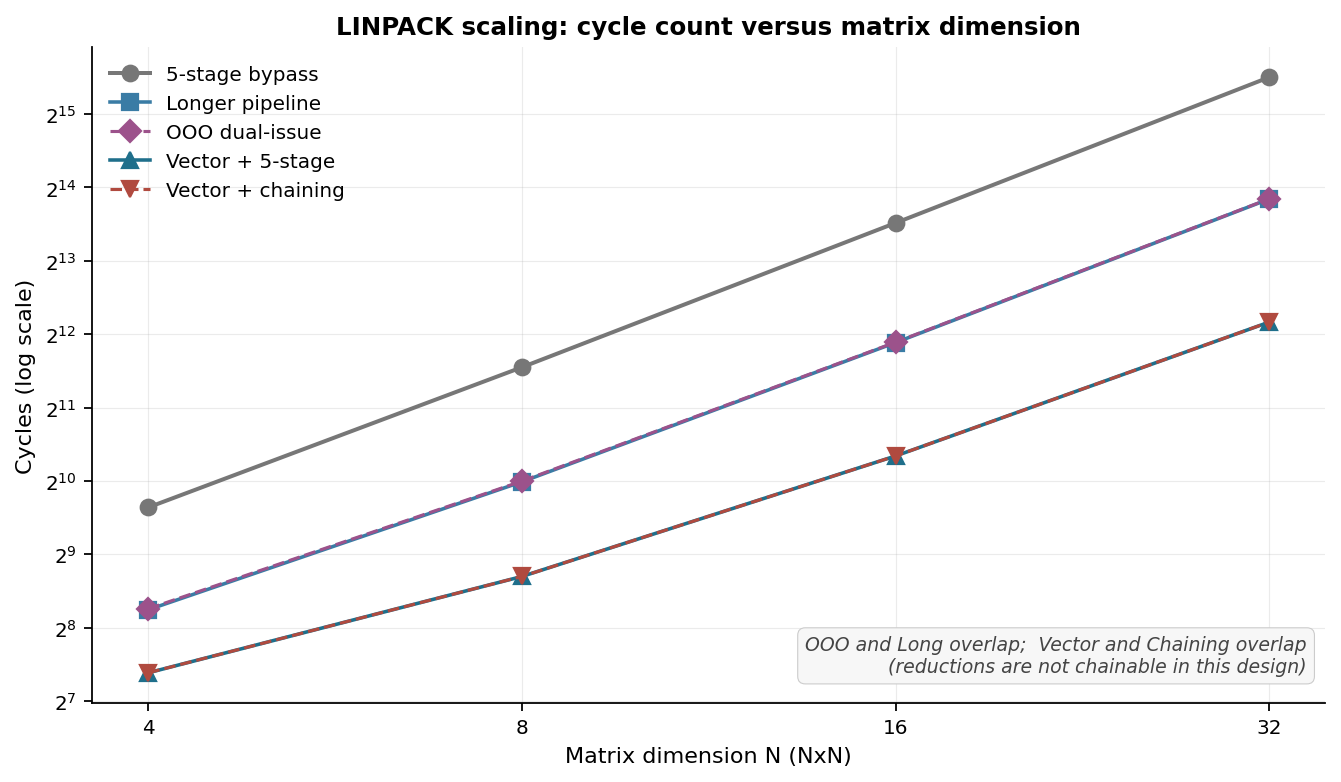
\includegraphics[width=\columnwidth]{media/linpack-scaling.png}}
\caption{LINPACK scaling. Vector and chained curves overlap because
LINPACK's inner loop ends in a reduction (which is not chainable in
this design); chaining cannot grab additional pairs.}
\label{fig:linpack_scaling}
\end{figure}

That overlap of the vector and chained curves on LINPACK shows that chaining cannot capture every dependent pair because
reductions do not chain in our design (their accumulator state would
break the lockstep dataflow assumption). LINPACK's hottest path goes
through a reduction, so the chained variant gets no benefit there.

\subsection{Chain depth study}
To isolate exactly the benefits of chaining, we wrote a 
microbenchmark of $N$ consecutive RAW-dependent VVADDs. Each instruction
reads the previous one's destination, with no other ops between them.
Fig.~\ref{fig:chain_depth} shows the result.

\begin{figure}[t]
\centerline{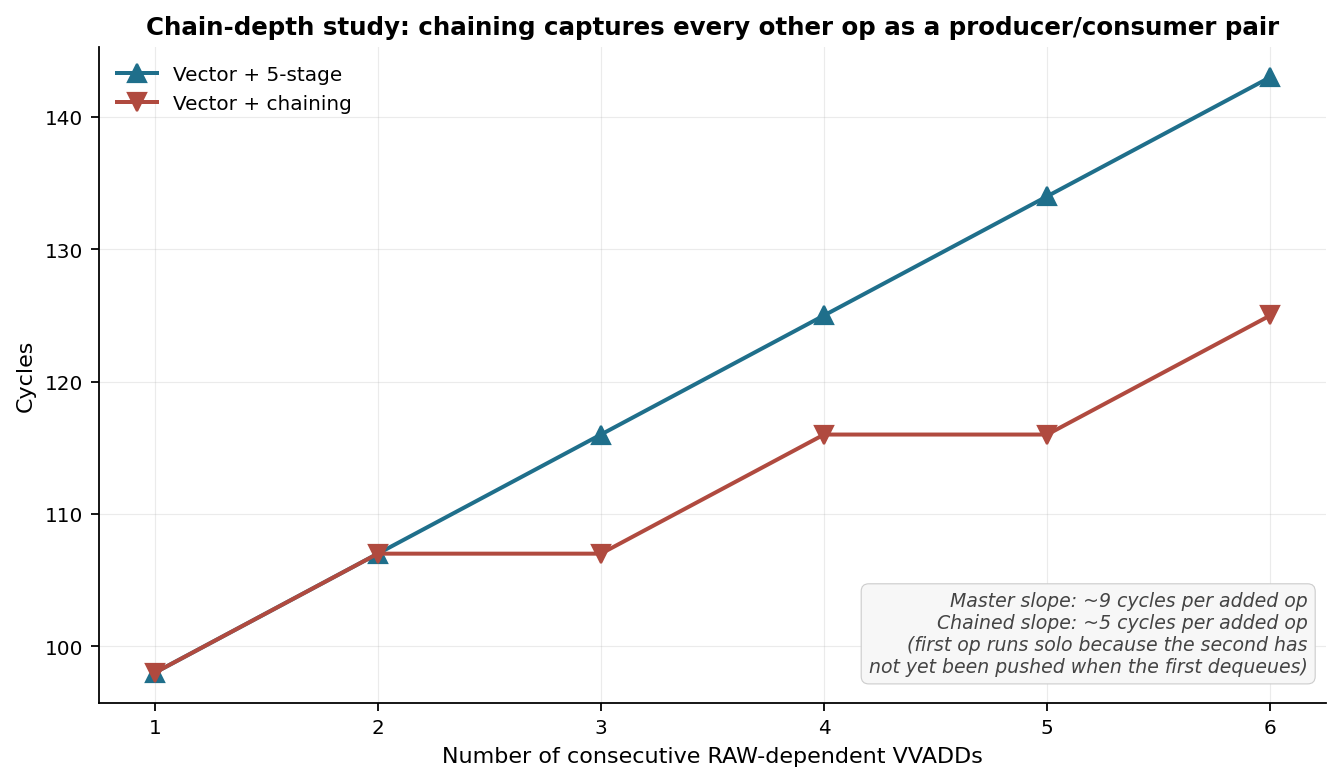
\includegraphics[width=\columnwidth]{media/chain-depth.png}}
\caption{Chain-depth study: $N$ consecutive RAW-dependent VVADDs.
The chained design adds roughly 5 cycles per added op vs.~9 cycles
for the baseline.}
\label{fig:chain_depth}
\end{figure}

The baseline cycle count scales as $\approx 9N + 89$, since each new
op adds one full chime ($\approx$ VL = 32 cycles, minus some overlap
of issue with the previous op's tail). The chained design scales as
$\approx 5N + 89$ on average, which halves the marginal cost because every other
new op is captured as the consumer of a chain pair and pays no new
chime. The staircase shape (depth 2 = depth 3, depth 4 = depth 5) is expected because the chained controller pulls in pairs, and
adding one op to an existing pair-aligned sequence costs nothing
until it forces a new pair.

\subsection{Command queue depth}
A separate sweep over command queue depths (2, 4, 8, 16) showed no
change in cycle count for any of our standard kernels. This is
because every kernel ends in VFENCE per strip-mined batch, draining
the queue before the scalar core gets far enough ahead to fill it.
The queue would matter for code patterns that pipeline scalar and
vector work without per-batch fences; our benchmark suite does not
contain such code and is left for future work.

\subsection{Energy considerations}
We did not synthesize the design or run a calibrated energy
simulation, so we explain a rough qualitative picture. Following the per-event energy model in
\cite{horowitz_isscc}, dynamic energy is dominated by per-instruction
overhead (fetch, decode, register-file read) which are roughly
70~pJ each in 28~nm CMOS, which is much larger than ALU operations
(~0.1~pJ). For a kernel like daxpy at $N = 32$, the dynamic
instruction count drops from 322 (scalar) to 44 (vector), so the
overhead component of energy is roughly expected to shrink by approximately 7$\times$,
even though the per-element compute and memory components are
unchanged. The cycle count reduction also reduces the leakage and
clock-tree component, but dynamic-overhead reduction is the
main source. A proper quantitative estimation study is left
as future work.

\section{Limitations and Future Work}
The most important limitations are: (1) the design has only one
lane, so peak throughput is one element per cycle and we cannot
exploit the multi-lane scaling described in
\cite[Fig.~4.5]{hp_book}; (2) VLMAX is fixed at 32 and longer
vectors require software strip-mining; (3) the ALU is integer-only,
so true floating-point AXPY is out of scope; (4) memory accesses
arbitrate one port between scalar and vector code, giving us no
gather/scatter and no parallel banks. Addressing the first two would
require parameterizing NUM\_LANES and the VRF dimensions, then
duplicating ALUs and partitioning the register file as in
\cite{hwacha}. A scoreboard would
extend chaining to non-adjacent dependent pairs.

We also acknowledge a gap in test coverage. Our tests and
benchmarks together span about half of the 32 instructions in
the ISA. The covered subset includes everything the benchmarks need (SETVL, VFENCE, CVM, VLW/VSW, VLWS/VSWS, VVADD, VVSUB, VVMUL, VSADD, VSMUL, VREDSUM) but leaves missing tests: the integer divide and remainder ops (VVDIV/VVREM/VSDIV/VSREM), the bitwise logical and shift family (VVAND/OR/XOR, VVSLL/SRL/SRA), the four remaining vector-scalar variants, the two other reductions (VREDAND, VREDOR), and the comparison/mask-setting instructions (VSEQ/SLT/SLE/SGT/SGE/SNE) are untested. The mask register and
predicated-write hardware is therefore unverified end-to-end. A follow-on test suite of one short program per opcode would
address this. We did not get to it inside the two-week budget.

\section{Conclusion}
We built and evaluated a decoupled vector coprocessor for the class
RISC-V core with a 32-instruction custom ISA, a 1~KiB vector register
file, and Cray-style chaining as an optional extension. Across six
data-parallel kernels we measured speedups of 1.9$\times$--9$\times$
over the 5-stage scalar baseline, with the largest performance improvements on
intense arithmetic kernels (LINPACK, dot-product) where loop
overhead dominates scalar runtime. A chain-depth microbenchmark
confirmed the chaining mechanism halves the marginal cost of
RAW-dependent pairs, exactly as predicted by the convoy/chime model
in \cite[\S 4.2]{hp_book}. The project demonstrates that even a
single-lane vector coprocessor captures most of the benefit of
vector architectures on the kinds of kernels our textbook describes,
and that chaining is straightforward to layer onto an existing
decoupled design with modest hardware additions (one extra read
port, one extra write port, a second ALU, and a forwarding mux).

\begin{thebibliography}{00}
\bibitem{hp_book} J.~L. Hennessy and D.~A. Patterson,
  \textit{Computer Architecture: A Quantitative Approach},
  6th ed. Morgan Kaufmann, 2017, Ch.~4.
\bibitem{cray1} R.~M. Russell, ``The CRAY-1 computer system,''
  \textit{Comm. ACM}, vol. 21, no. 1, pp. 63--72, Jan. 1978.
\bibitem{smith_dae} J.~E. Smith, ``Decoupled access/execute computer
  architectures,'' \textit{ACM Trans. Comput. Syst.}, vol. 2, no. 4,
  pp. 289--308, Nov. 1984.
\bibitem{avx_isa} Intel Corporation, \textit{Intel 64 and IA-32
  Architectures Software Developer's Manual}, vol. 1, ch. 14
  (Advanced Vector Extensions), 2023.
\bibitem{nvidia_fermi} NVIDIA Corporation, ``NVIDIA's next generation
  CUDA compute architecture: Fermi,'' Whitepaper, 2009.
\bibitem{rvv} K.~Asanovi\'c \textit{et al.}, ``RISC-V `V' Vector
  Extension Specification,'' RISC-V International, version 1.0,
  2021.
\bibitem{hwacha} Y.~Lee \textit{et al.}, ``A 45nm 1.3GHz 16.7
  double-precision GFLOPS/W RISC-V processor with vector
  accelerators,'' in \textit{ESSCIRC}, 2014, pp. 199--202.
\bibitem{ara} M.~Cavalcante \textit{et al.}, ``Ara: A 1-GHz+ scalable
  and energy-efficient RISC-V vector processor with multiprecision
  floating-point support in 22-nm FD-SOI,'' \textit{IEEE Trans.
  VLSI Syst.}, vol. 28, no. 2, pp. 530--543, Feb. 2020.
\bibitem{horowitz_isscc} M.~Horowitz, ``Computing's energy problem
  (and what we can do about it),'' in \textit{IEEE Int.~Solid-State
  Circuits Conf. (ISSCC)}, 2014, pp. 10--14.
\end{thebibliography}

\end{document}
